%%%%%%%%%%%%%%%%%%%%%%%%%%%%%%%%%%%%%%%%%
% Arsclassica Article
% LaTeX Template
% Version 1.1 (10/6/14)
%
% This template has been downloaded from:
% http://www.LaTeXTemplates.com
%
% Original author:
% Lorenzo Pantieri (http://www.lorenzopantieri.net) with extensive modifications by:
% Vel (vel@latextemplates.com)
%
% License:
% CC BY-NC-SA 3.0 (http://creativecommons.org/licenses/by-nc-sa/3.0/)
%
%%%%%%%%%%%%%%%%%%%%%%%%%%%%%%%%%%%%%%%%%

%----------------------------------------------------------------------------------------
%	PACKAGES AND OTHER DOCUMENT CONFIGURATIONS
%----------------------------------------------------------------------------------------

\documentclass[
article,
10pt, % Main document font size
oneside, % One page layout (no page indentation)
BCOR5mm, % Binding correction
]{scrartcl}
\usepackage[a4paper,margin=3cm]{geometry}
\usepackage[italian]{babel}
\usepackage[utf8]{inputenc}
\usepackage{atbegshi}% http://ctan.org/pkg/atbegshi
\usepackage{tikz}
\usetikzlibrary{shapes}
\usepackage{amsmath}
\usepackage{xspace}
\usepackage[usestackEOL]{stackengine}
\usepackage{graphicx}
\usepackage{caption}
\usepackage{subcaption}
\usepackage{float}
\newcommand{\A}{\ensuremath{\mathcal{A}}\xspace}
\newcommand{\B}{\ensuremath{\mathcal{B}}\xspace}
\newcommand\pa[1]{\ensuremath{\left(#1\right)}}
\AtBeginDocument{\AtBeginShipoutNext{\AtBeginShipoutDiscard}}

\hyphenation{Fortran hy-phen-ation} % Specify custom hyphenation points in words with dashes where you would like hyphenation to occur, or alternatively, don't put any dashes in a word to stop hyphenation altogether

%----------------------------------------------------------------------------------------
%	TITLE AND AUTHOR(S)
%----------------------------------------------------------------------------------------

\begin{document}

\begin{center}
\title{
  \begin{figure}[h!]
  \centering
  
\includegraphics[width=.3\columnwidth]{images/project_logo.png}
  \end{figure}
  Bike Sharing Demand \\
  Progetto di \textbf{Data Mining}
}
\author{
Sebastiano Valle 1050123}
\end{center} % The article author(s) - author affiliations need to be specified in the AUTHOR AFFILIATIONS block






%\date{} % An optional date to appear under the author(s)

%----------------------------------------------------------------------------------------

%----------------------------------------------------------------------------------------
%	TABLE OF CONTENTS & LISTS OF FIGURES AND TABLES
%----------------------------------------------------------------------------------------

\maketitle % Print the title/author/date block

\setcounter{page}{1} % Set the depth of the table of contents to show sections and subsections only


\raggedright{}
\newpage{}
\tableofcontents % Print the table of contents



\listoffigures % Print the list of figures

\listoftables % Print the list of tables

\section{Introduzione}

\subsection{Abstract}
Il progetto consiste nell'analisi di dati riguardanti il \emph{Bike sharing}.
Il \emph{Bike sharing} è un servizio che viene fornito nelle principali città,
tramite il quale è possibile utilizzare una bici prelevandola da un chiosco
multimediale e riportandola ad un altro chiosco una volta terminato l'utilizzo.

In questo modo le persone possono spostarsi per la città in base ad esigenze
impreviste, senza aver doversi muovere con la propria bici, cosa
particolarmente scomoda se per raggiungere il posto in cui serve
effettivamente utilizzare la bici bisogna utilizzare un servizio pubblico come
autobus o treno.

Naturalmente, questi spostamenti possono risultare molto interessanti per i
\emph{data scientist} poichè (ad esempio) forniscono dati su:

\begin{itemize}
\item durata del viaggio;
\item luoghi di partenza più ricorrenti;
\item luoghi di arrivo più ricorrenti.
\end{itemize}

Questa possibilità di ottenere dati in un modo molto semplice ha spinto gli
stessi ricercatori ad analizzare la richiesta del servizio di \emph{Bike
sharing}, così da poter prevedere le possibili quantità di dati disponibili.

\subsection{Dati utilizzati}\label{sec:intro-dati}

I dati utilizzati provengono da un contest su
Kaggle\footnote{\texttt{https://www.kaggle.com/c/bike-sharing-demand}},
che a sua volta li ha recuperati dal repository del corso di
\emph{Machine Learning} dell'\textbf{University of California, Irvine}.

Sono disponibili due set, uno per l'addestramento (che chiameremo anche
\emph{training set}) e uno (il \emph{test set}) su cui fare previsioni
utilizzando il modello ``migliore'' ottenuto grazie all'analisi del training
set.

Tuttavia, il test set non verrà utilizzato poichè esso non contiene i valori
``veri'' delle variabili risposta e da qui in poi l'unico dataset a cui ci
riferiremo sarà il \textbf{training set}.

Il dataset fornito presenta le seguenti variabili:

\begin{itemize}
\item \textbf{Variabili esplicative}:
  \begin{itemize}
  \item \texttt{datetime}: variabile che presenta valori del tipo ``YYYY-MM-AA
    HH:MM:SS'', ovvero la data in formato americano seguita dall'orario
    giornaliero

  \item \texttt{season}: variabile qualitativa che assume i seguenti valori:
    \begin{itemize}
    \item \textbf{1}: primavera
    \item \textbf{2}: estate
    \item \textbf{3}: autunno
    \item \textbf{4}: inverno
    \end{itemize}

  \item \texttt{holiday}: variabile qualitativa che può valere \textbf{1}
  (giorno festivo) o \textbf{0} (giorno non festivo):

  \item \texttt{working day}: variabile qualitativa che può valere \textbf{1}
  (giorno feriale) o \textbf{0} (giorno non feriale):

  \item \texttt{weather}: variabile qualitativa che assume i seguenti
    valori:
    \begin{itemize}
    \item \textbf{1}: terso, con poche nuvole o parzialmente nuvoloso
    \item \textbf{2}: nebbia con possibili nuvole
    \item \textbf{3}: pioggia
    \item \textbf{4}: temporale, neve o grandine
    \end{itemize}

  \item \texttt{temp}: temperatura reale in gradi Celsius

  \item \texttt{atemp}: temperatura percepita in gradi Celsius

  \item \texttt{humidity}: umidità relativa (in percentuale)

  \item \texttt{windspeed}: velocità del vento

  \end{itemize}
\item \textbf{Variabili risposta}:
    \begin{itemize}

  \item \texttt{casual}:  biciclette noleggiate da utenti non registrati

  \item \texttt{registered}: biciclette noleggiate da utenti registrati

  \item \texttt{count}: totale delle biciclette noleggiate

    \end{itemize}
\end{itemize}
 % 100%
\section{Primo approccio: modello lineare}

\subsection{Workspace}

Prima di iniziare a parlare del modello adottato per prevedere la richiesta di
\emph{Bike sharing}, è opportuno chiarire come verranno gestite le variabili
coinvolte durante l'analisi dei dati.

\subsubsection{Variabili esplicative}\label{sec:modlin-work-espl}
Per quanto riguarda le variabili esplicative, \texttt{holiday},
\texttt{working day}, \texttt{weather}, \texttt{temp}, \texttt{atemp},
\texttt{humidity}, \texttt{windspeed} non verranno trasformate in alcun modo.
In particolare:

\begin{itemize}
\item \texttt{holiday}, pur essendo qualitativa, è già espressa in un formato
  accettabile, ovvero \textbf{0} per una modalità (\textbf{N}) e \textbf{1}
  per l'altra (\textbf{S});
\item il caso di \texttt{workingday} è totalmente analogo a quello di
  \texttt{holiday};
\item \texttt{weather}, pur prevedendo quattro modalità, si può vedere come
  una variabile quantitativa per la quale più alto è il valore, peggiore è il
  tempo (con valori compresi tra quelli nominati nella sezione
  \ref{sec:intro-dati}).
\end{itemize}

\paragraph{Variabili trasformate} \mbox{}\\
Non tutte le variabili in gioco erano fornite in modo tale da essere
analizzate con semplicità.
Le restanti variabili esplicative sono state impostate con i seguenti criteri:

\begin{itemize}
\item \texttt{datetime} conteneva al suo interno il giorno e l'ora.
  Dopo una rapida analisi del dataset, si è notato che tutte le ore erano in
  realtà nel formato ``HH:00:00'', deducendo che si trattasse di misurazioni
  orarie. \\
  Oltre a ciò è stato considerato che la richiesta del servizio di \emph{Bike
  sharing} non dipende fortemente da un giorno particolare (e.g. 2012-07-04),
  ma principalmente dalla stagione a cui questo apparteneva e al fatto che
  questo fosse festivo e/o feriale o meno, fattori già presenti in altre
  variabili esplicative. \\
  A maggior ragione, lo scopo finale del modello era quello di effettuare
  previsioni su giorni non presenti nel dataset, perciò riuscire a costruire
  un modello che restituisse previsioni corrette su un giorno di cui si
  conoscevano già i risultati non era significativo, mentre il trend con cui
  il servizio viene richiesto durante una giornata potrebbe esserlo.\\
  Di conseguenza, si è ritenuto opportuno trasformare \texttt{datetime} in una
  variabile con valori interi uguali ad HH (ignorando completamente il
  giorno), con valori perciò compresi tra 0 (mezzanotte) e 23 (11:00 PM);
\item \texttt{season} presentava quattro possibili modalità. A differenza di
  \texttt{weather}, le cui modalità potevano essere viste come un insieme
  ordinato, non si vede alcun ordine per le stagioni. \\
  Un possibile tentativo sarebbe stato, in modo del tutto analogo a
  \texttt{weather}, pensare a un insieme dove al valore minimo sarebbe
  corrisposta la stagione caratterizzata da temperature più fredde e da
  condizioni metereologiche peggiori e viceversa per il valore massimo. \\
  Tuttavia, questo approccio non è stato considerato valido poichè primavera e
  autunno sono simili da questo punto di vista. \\
  Si è proceduto creando due nuove variabili, \texttt{season.summer} e
  \texttt{season.fall}, così che la variabile originaria \texttt{summer} fosse
  riorganizzata nel seguente modo:
  \begin{itemize}
  \item \texttt{season} variabile che vale 1 se la stagione è primavera
    (modalità \textbf{1} per la variabile originaria)
  \item \texttt{season.summer} variabile che vale 1 se la stagione è primavera
    (modalità \textbf{2} per la variabile originaria)
  \item \texttt{season.fall} variabile che vale 1 se la stagione è primavera
    (modalità \textbf{3} per la variabile originaria)
  \item  \texttt{season}, \texttt{season.summer} e \texttt{season.fall} con
    valore 0 se la stagione è inverno (modalità \textbf{4} per la variabile
    originaria)
  \end{itemize}
\end{itemize}

Tali trasformazioni sono state applicate durante il popolamento del dataset, il
cui script è stato riportato in sezione \ref{sec:script-populate}.

In fondo allo script si possono notare alcune costanti che vengono settate per
il workspace: si tratta di \texttt{columns}, ovvero il nome delle variabili
esplicative utilizzate, e di altre costanti il cui uso verrà spiegato più
dettagliatamente in seguito.

\subsubsection{Variabili risposta}
Per le variabili risposta, è stato scelto di considerare solo
\texttt{train\$count}, poichè lo studio dei modelli per le variabili
\texttt{train\$registered} e \texttt{train\$casual} è del tutto analogo a
quello della variabile che insieme compongono.

\subsection{Modello lineare}
Dopo aver impostato correttamente il workspace, si può procedere calcolando il
modello lineare semplice $ y = \beta{}_0 + \beta{}_1 \cdot{} x + \epsilon{} $
per tutte le variabili, dove y è train\$count e x una delle variabili
esplicative.
Inizialmente questa operazione viene ripetuta con il comando \texttt{train.lm
= lm(y $ \sim{} $ x)} per tutte le variabili esplicative, ottenendo il
risultato migliore per x = train\$datetime.

Questo risultato ci può dare garanzie sulla buona intuizione riguardo il
formato scelto per la variabile \texttt{datetime}, spiegato nella sezione
\ref{sec:modlin-work-espl}, ovvero che l'ora è uno dei fattori che incidono
molto sulla richiesta del servizio di \emph{Bike sharing}.

Tale considerazione può essere compresa guardando i valori dei residui visibili
grazie alla visione d'insieme del modello lineare fornita dal comando
\texttt{summary()}.

\begin{figure}[H]\label{fig:simplest-linear-model}
  \centering
  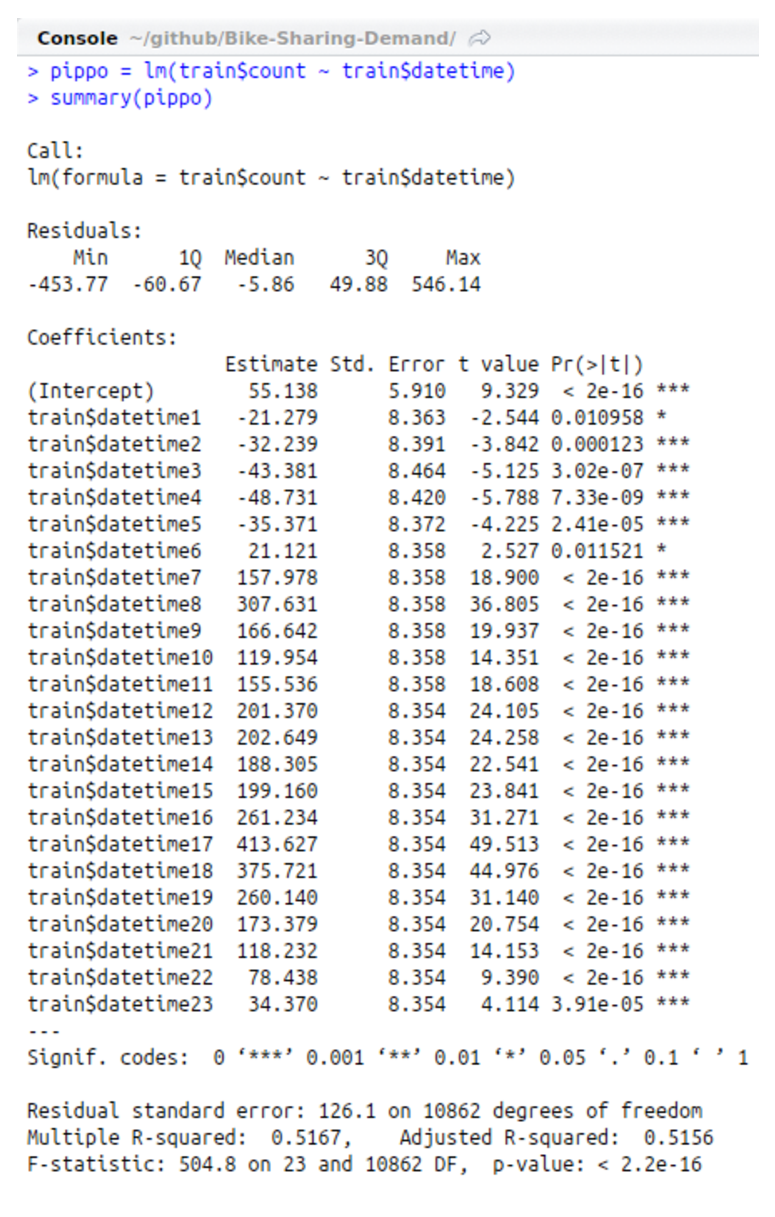
\includegraphics[width=.7\columnwidth]{images/simplest-linear-model.eps}
  \caption{Modello lineare con \texttt{train\$datetime}}
\end{figure}

I dati relativi al modello lineare appena individuato potrebbero ingenuamente
suggerire che la stima individuata per il coefficiente $\beta{}_1$ sia buona,
visto un valore molto elevato della statistica F e, di conseguenza, un p-value
prossimo a 0.

Tuttavia, richiedendo i grafici relativi al modello lineare, è ben facile
intuire che il modello lineare calcolato non è affatto soddisfacente, poichè è
evidente che gli errori non seguono distribuzione normale secondo
questo modello:

\begin{itemize}
\item I residui, sebbene abbiano media nulla, non sembrano omoschedastici;
  oltre a questo, pare anche che il modello non riesca a cogliere una
  curvatura presente nella variabile risposta;
\item Dal QQPlot si vede facilmente che la curva si discosta notevolmente
  rispetto alla distribuzione dei quantili di una distribuzione normale.
\end{itemize}

\begin{figure}[H]
  \centering
  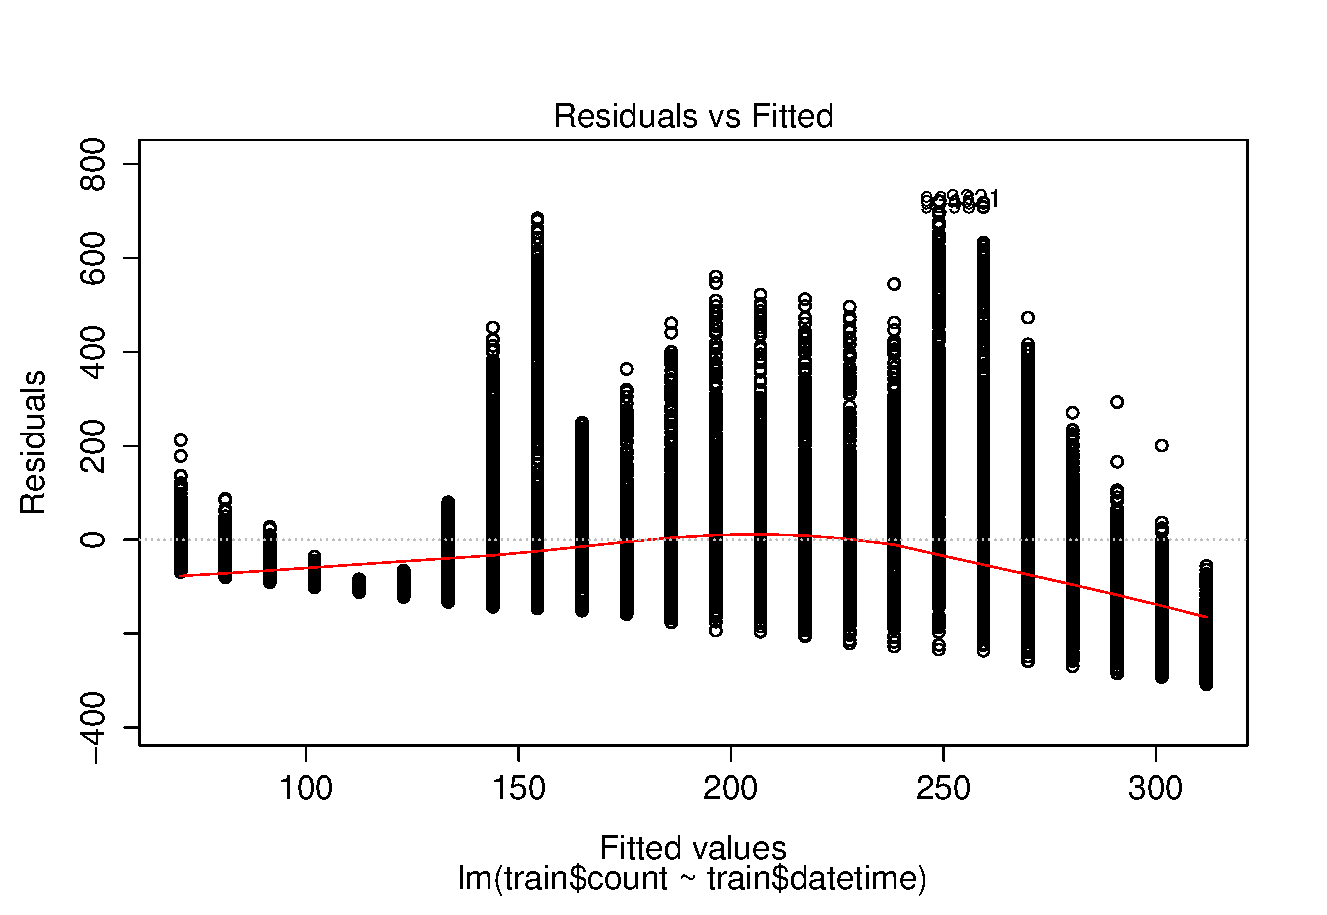
\includegraphics[width=.7\columnwidth]{images/simple-linear-model-plot.eps}
  \caption{Grafico dei residui per il modello lineare con
  \texttt{train\$datetime}}\label{fig:simpl-mod-lin-residuals}
\end{figure}

\begin{figure}[H]
  \centering
  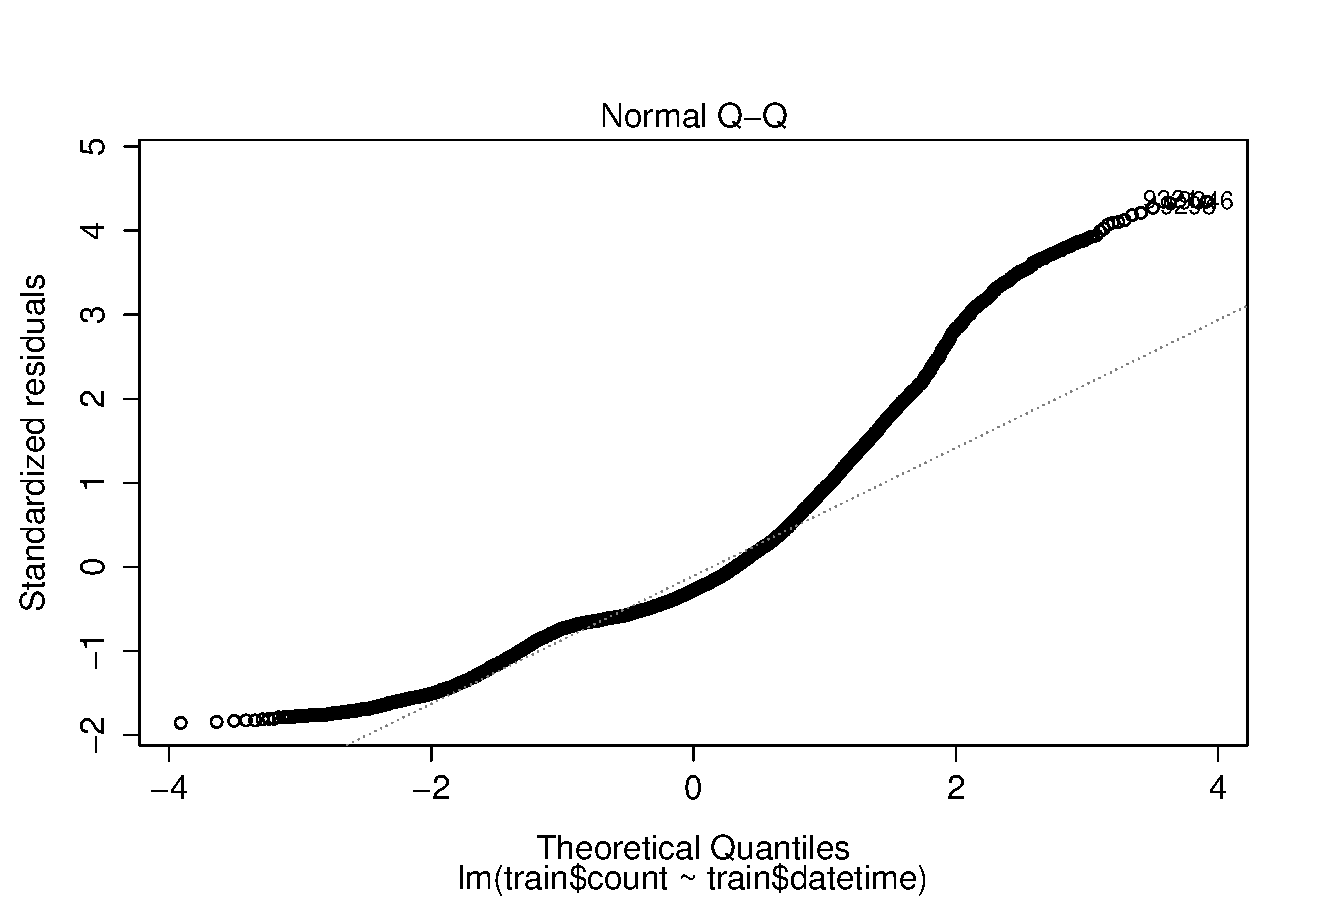
\includegraphics[width=.7\columnwidth]{images/simplest-linear-model-qqplot.eps}
  \caption{QQPlot per il modello lineare con
  \texttt{train\$datetime}}\label{fig:simpl-mod-lin-qqplot}
\end{figure}

\paragraph{Modelli con variabili esplicative trasformate} \mbox{}\\
Per rimediare a quanto detto sopra, si pensa a come introdurre nel modello
qualcosa che contribuisca a rendere la distribuzione degli errori più simile
a quella gaussiana.

Tale procedimento è totalmente giustificato dal fatto che si ritiene di poter
approssimare la variabilità di un comportamento umano come l'utilizzo del
\emph{Bike sharing} con una distribuzione normale.

Inizialmente il tentativo consiste nell'utilizzare un modello del tipo
$ y = \beta{}_0 + \beta{}_1 \cdot{} z + \epsilon{} $, dove z è la variabile
\texttt{train\$datetime} elevata al quadrato.

Questa strada però non porta i risultati desiderati: nella figura
\ref{fig:simpl-mod-lin-residuals} era ben visibile che i residui non erano
soddisfacenti poichè ``sbagliavano'' per eccesso. Infatti vi erano errori
significativi di sovrastima, mentre le sottostime erano numerose ma di valore
più contenuto.

Analizzando il modello ottenuto, si può infatti vedere che:

\begin{itemize}
\item l'errore standard dei residui è aumentato;
\item il grafico dei residui è molto simile a quello visto nel primo studio;
\item i quantili osservati per i residui si discostano ancora di molto da
  quelli di una distribuzione normale.
\end{itemize}

\paragraph{Modelli con variabili risposta trasformate} \mbox{}\\
Si procede dunque con un secondo tentativo, provando ad agire sul valore della
variabile risposta. Dagli stadi di analisi precedenti ormai è chiaro che
l'errore commesso era dovuto ad alcuni valori della variabile risposta che
erano piuttosto elevati.

Anzichè trasformare le variabili esplicative, quindi, forse è più conveniente
trasformare la variabile risposta in modo da attenuare i valori più alti di
questa:

\centering $ w = \beta{}_0 + \beta{}_1 \cdot{} x + \epsilon{} $
\flushleft dove $ w = log(y) $.

Questo modello risulta vincente, poichè l'errore standard dei residui passa da
166 a 1.333 e il grafico dei residui risulta più adeguato rispetto ad una
distribuzione normale, così come il QQPlot ora ha una distribuzione dei
quantili osservati molto più vicina a quella di una normale.

\begin{figure}[H]
  \centering
  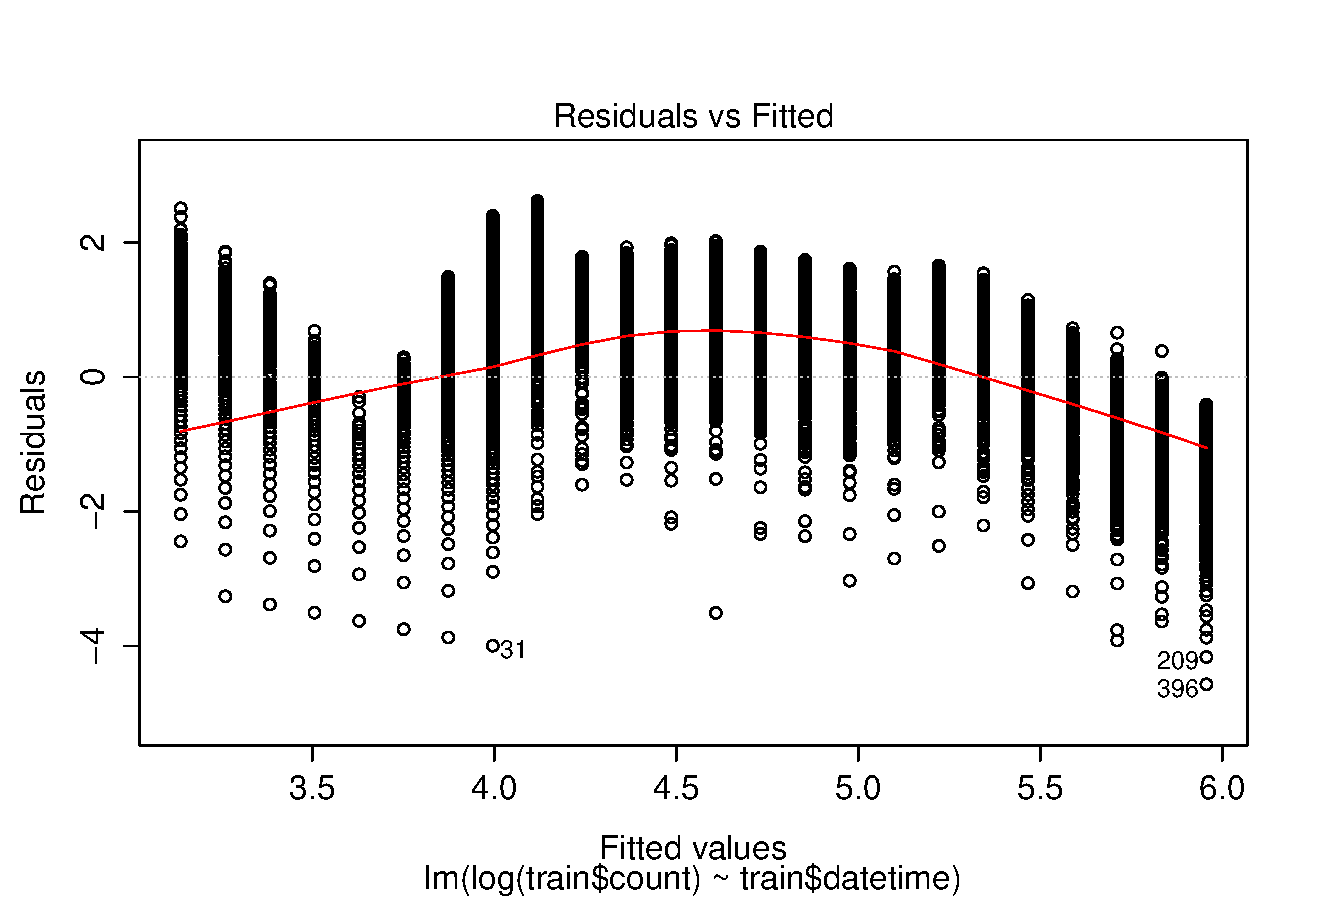
\includegraphics[width=.7\columnwidth]{images/simple-lm-log-residuals.eps}
  \caption{Grafico dei residui per il modello lineare migliorato con
  \texttt{train\$datetime}}\label{fig:simpl-lm-log-residuals}
\end{figure}

\begin{figure}[H]
  \centering
  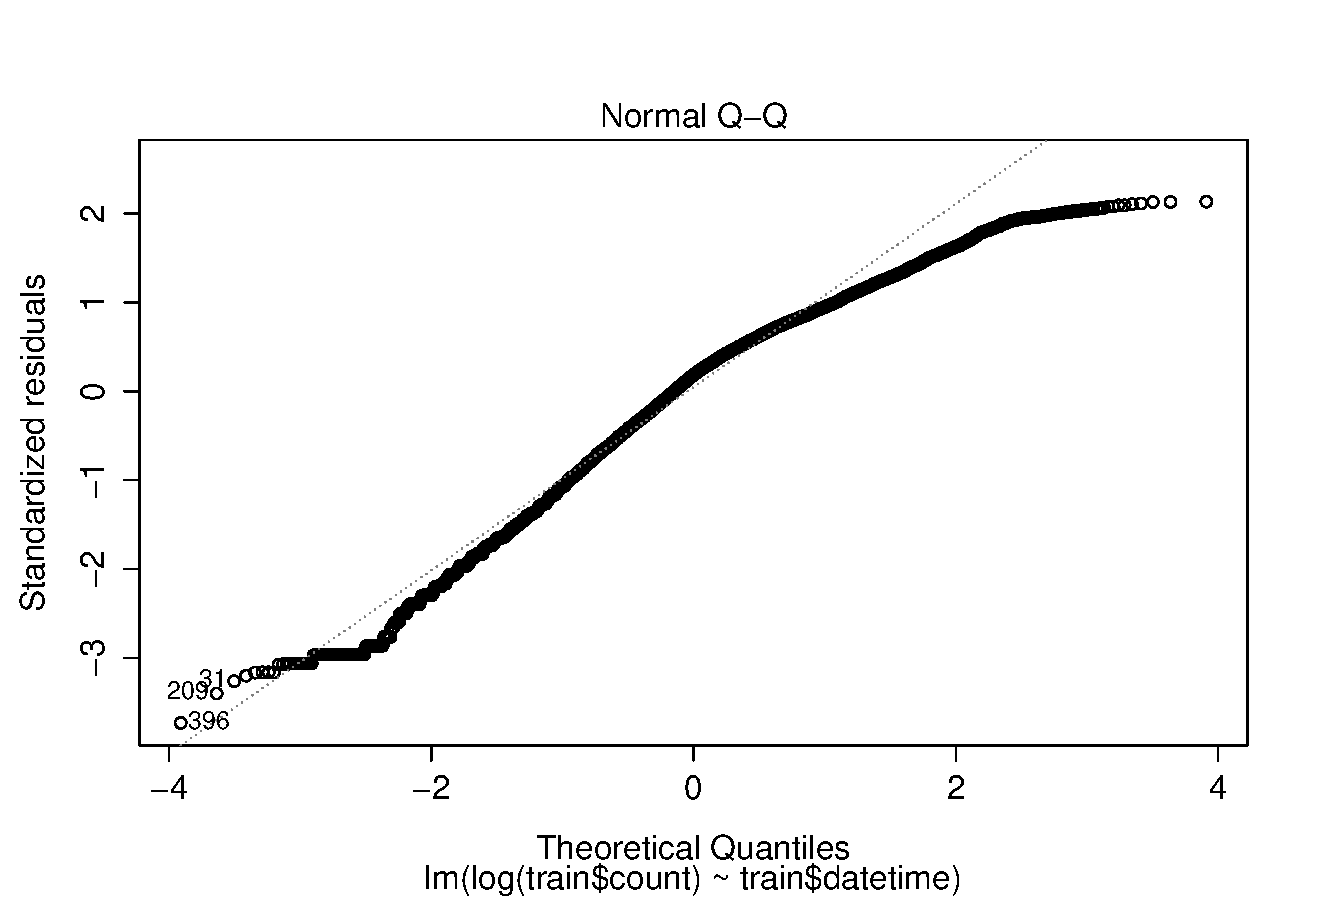
\includegraphics[width=.7\columnwidth]{images/simple-lm-log-qqplot.eps}
  \caption{QQPlot per il modello lineare migliorato con
  \texttt{train\$datetime}}\label{fig:simpl-lm-log-qqplot}
\end{figure}

\subsection{Modello lineare con \emph{forward stepwise selection}}
Il modello di prima ha portato a discreti risultati, se non per il fatto che
utilizzava solamente una delle variabili esplicative.

Un approccio naïf potrebbe essere quello di inserire nel calcolo del modello
lineare tutte le variabili esplicative presenti nel set \texttt{train} e di
calcolare il modello lineare con il comando fornito da R.

Come è possibile vedere, ci sono alcune variabili che non sono significative e
altre che invece è sensato che appartengano al nostro modello:

\begin{figure}[H]
  \centering
  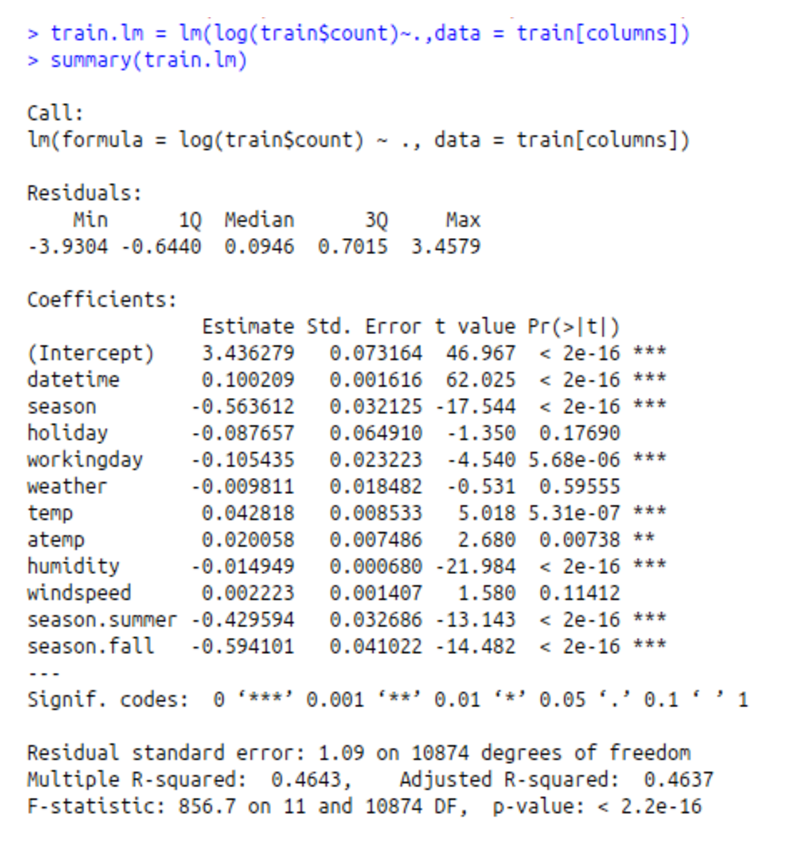
\includegraphics[width=.55\columnwidth]{images/lm-with-all-vars.eps}
  \caption{Modello lineare calcolato su tutte le variabili in modo
    non-ordinato}\label{fig:simpl-lm-log-qqplot}
\end{figure}

Tuttavia, anzichè provare manualmente qualsiasi combinazione di variabili
affinchè non si trovi il modello lineare migliore, si decide di automatizzare
il tutto con un paio di script:

\begin{itemize}
\item \texttt{linearModel.R} (sez. \ref{sec:script-linear-model}): questo
  script in pratica realizza quanto fatto nella prima parte dell'analisi
  tramite un modello lineare.
  \begin{enumerate}
  \item Dato il modello $ w = \beta{}_0 + \beta{}_1 \cdot{} x + \epsilon{} $,
  viene cercata la variabile esplicativa più significativa, confrontando la
  statistica F delle variabili \texttt{train\$[columns]} (ovvero le variabili
  esplicative);
  \item Nel frattempo, vengono stampate a video le variabili esplicative, il
  coefficiente di determinazione e la statistica F ottenuti usando questi come
  ``x'' per il modello;
  \item A questo punto, viene trovata la variabile più significativa, tale
  risultato viene stampato a video e questa viene usata per calcolare il
  miglior modello lineare con una variabile esplicativa;
  \item Il nome di questa variabile viene salvato in un array chiamato
  \texttt{already\_present} e viene invocato il secondo script.
  \item Alla fine dello script, il workspace viene pulito, lasciando solamente
  le variabili \texttt{train.lm} (il modello ricercato) e \texttt{train.lm2}
  (il modello con tutte le variabili esplicative oppure con una variabile non
  significativa presente oltre a quelle presenti in \texttt{train.lm}).
  \end{enumerate}
\item \texttt{linear\_model\_forward\_steps.R} (sez.
  \ref{sec:script-linear-model-fwd-steps}): questo script serve per iterare
  lungo le variabili esplicative al fine di inserire in modo incrementale le
  variabili più significative per il nostro modello.
  \begin{enumerate}
  \item All'inizio dello script, \texttt{train.lm} è il modello lineare con n
    variabili esplicative, dove n è il numero di volte che è stato invocato;
  \item Per ognuna delle variabili esplicative, viene eseguito un insieme di
    istruzioni. Se la variabile è già presente nel modello (e quindi in
    \texttt{already\_present}), viene saltata;
  \item Si procede calcolando il modello lineare aggiungendo alle variabili
    già presenti quella coinvolta nell'iterazione corrente;
  \item Viene eseguita l'ANalysis Of VAriance (\textbf{ANOVA}) sul nuovo
    modello;
  \item Tramite queste iterazioni, si trova la variabile più significativa da
    aggiungere al modello lineare presente all'inizio dello script;
  \item Tale variabile viene inserita solamente se contribuisce in modo
      significativo a migliorare il modello; per far questo, si confronta il
      suo p-value con una soglia stabilita a priori (nel nostro caso 5\%),
      impostata con lo script di popolamento (sez. \ref{sec:script-populate})
      nella costante \texttt{FWD\_SW\_THRESHOLD};
    \item Se la variabile è stata inserita, viene ricalcolato \texttt{train.lm}
      aggiungendo questa variabile, vengono stampate le variabili presenti nel
      modello e viene invocato ricorsivamente questo script;
    \item Quando non vi sono più variabili da aggiungere, il workspace viene
      pulito (facendo attenzione a non ripetere rimozioni su oggetti già
      cancellati) e in \texttt{train.lm} è presente il modello ricercato.
  \end{enumerate}
\end{itemize}

Di seguito vengono riportati i dati del modello lineare ottenuto tramite gli
script sopra descritti:

\begin{figure}[H]
  \centering
  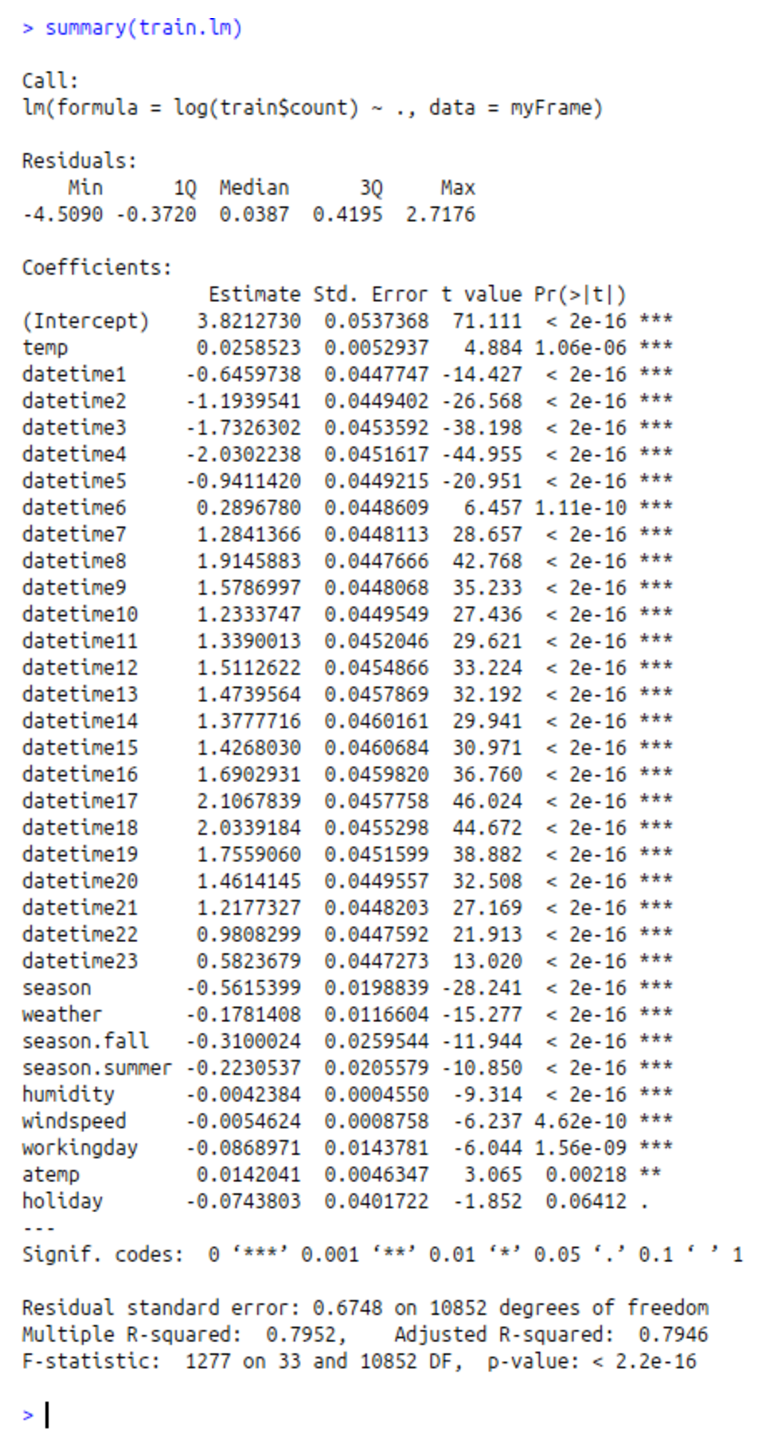
\includegraphics[width=.55\columnwidth]{images/lm-after-fwd-steps.eps}
  \caption{Modello lineare calcolato tramite forward-stepwise selection}
    \label{fig:simpl-lm-log-qqplot}
\end{figure}
 % 100%
\section{Metodi non lineari}\label{sec:non-linear}

Nella sezione \ref{sec:linear-model} sono stati introdotti ed adottati dei
metodi di regressione lineare che fornivano dei risultati discreti in prima
analisi, ma che possono essere sostituiti con modelli non lineari che spiegano
ancora meglio i dati.

A tal fine, sono stati provati vari modelli, descritti nelle sottosezioni
seguenti.

\subsection{Regressione locale}\label{sec:local-regression}
Come primo modello non lineare si sceglie di utilizzare la regressione locale,
servendosi del package \texttt{sm} presente in R.

In questo caso ci si limita a eseguire la regressione locale solamente per le
due variabili \texttt{datetime} e \texttt{temp}, le quali ci si aspettava che
fossero più importanti per la richiesta del servizio di \emph{Bike sharing};
tale ipotesi è stata verificata grazie al modello lineare, in cui queste
variabili erano risultate più significative sia nella scala logaritmica che in
quella originale.

Oltre a questo, la regressione locale viene svolta solamente per la scala
logaritmica, poichè si ritiene che riesca a modellare meglio il sistema in
esame.

\paragraph{Scelta di \emph{h}} \mbox{}\\
Per questo modello era importante scegliere il parametro \emph{h}, che regola
l'ampiezza della finestra di lisciamento.

Per la scelta del parametro, gli script \texttt{mySM\_temp.R} (sez.
\ref{sec:mySM-temp}) e lo script \texttt{mySM\_datetime.R} (non riportato
perchè pressochè uguale a quello per la variabile \texttt{temp}) sono stati
fatti girare più volte, ottenendo ogni volta una misura ottimale di h e
restringendo l'intervallo attorno al valore salvato in \texttt{optimal\_h}.

Di seguito viene riportato l'andamento dell'errore in funzione di h:

\begin{figure}[H]
  \centering
  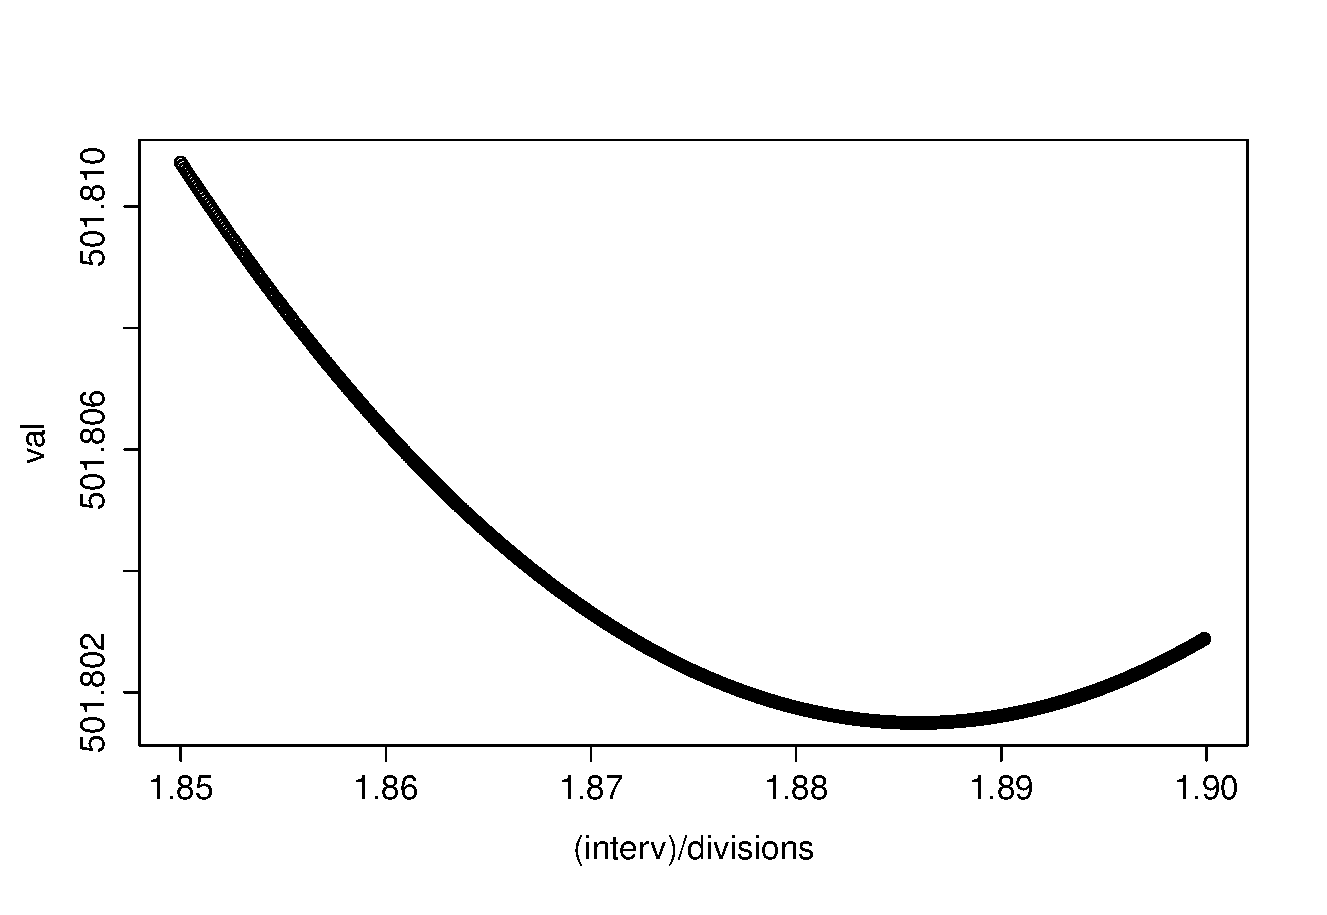
\includegraphics[width=.7\columnwidth]{images/non-linear/sm-optimal-h.eps}
  \caption{Curva dell'errore in funzione del parametro h}
  \label{fig:sm-optimal-h}
\end{figure}

Una volta iterato il procedimento fino ad avere una precisione per l'h
``ottimo'' migliore di $ \frac{1}{1000} $, si procede a disegnare la curva
grazie allo script \texttt{drawOptimalSM\_temp.R} (sez. \ref{sec:drawSM-temp}):

\begin{figure}[H]
  \centering
  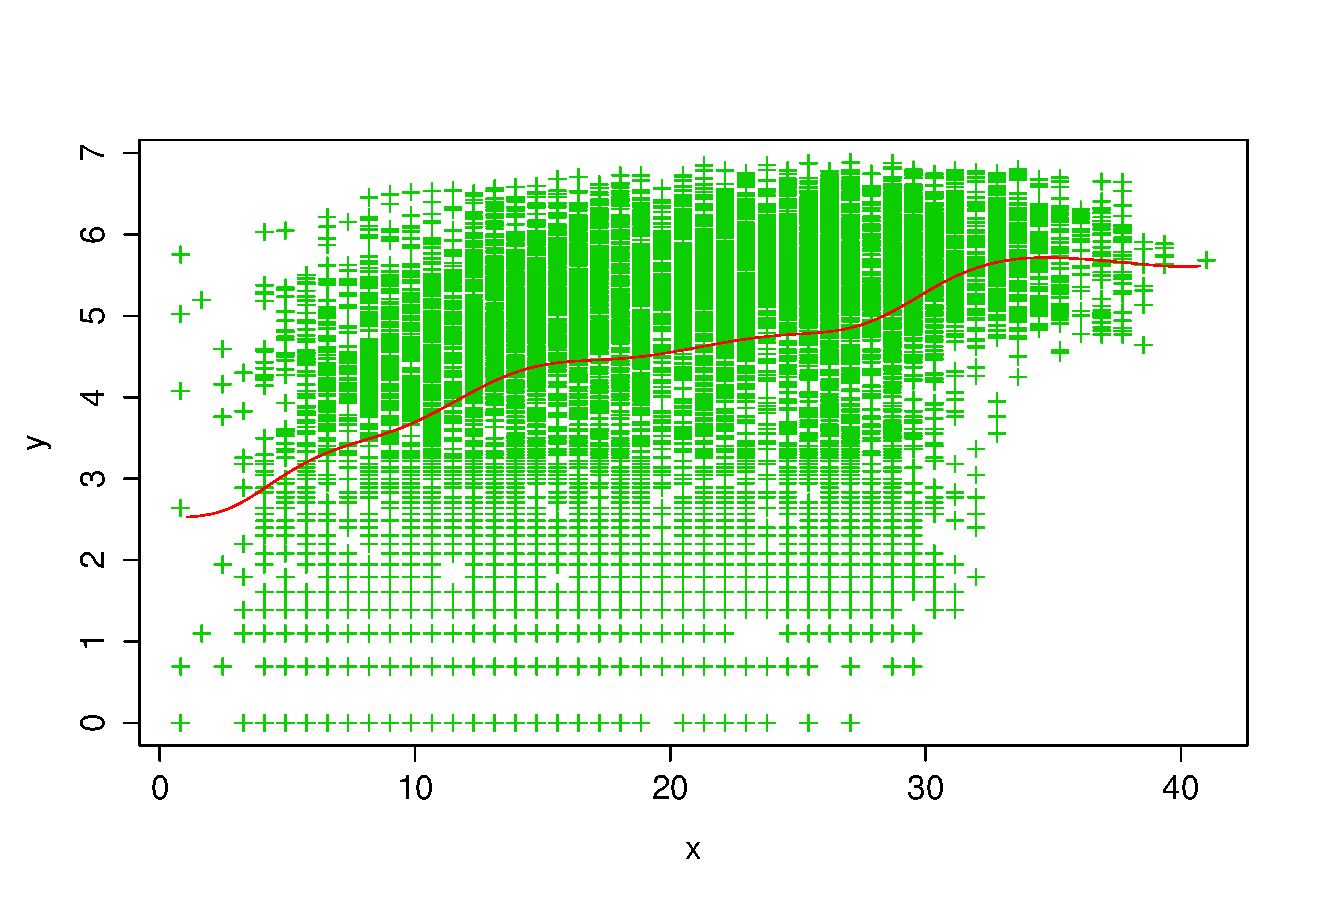
\includegraphics[width=.7\columnwidth]{images/non-linear/sm-draw.eps}
  \caption{Curva di regressione locale disegnata con il miglior h}
  \label{fig:sm-draw}
\end{figure}

\subsection{Loess}\label{sec:loess}
Un metodo molto simile al precedente, sempre di regressione locale, è il
\emph{loess}.

Questa tecnica permette di attenuare gli effetti degli \emph{outliers}, poichè
considera un intorno di k \emph{punti} e non un intorno di \emph{ampiezza} h.
Grazie a questa sua particolarità, il \emph{loess} è ritenuto un estimatore
\textbf{robusto}.

Tuttavia, anche questa tecnica viene eseguita con poche variabili alla volta;
sebbene il numero massimo di \emph{covariates} che il comando \texttt{loess}
di R accetta sia 4, si ritiene che eseguire la regressione locale con una
sola variabile esplicativa ne favorisca interpretazione.

Gli script utilizzati sono \texttt{loess\_temp.R} (sez. \ref{sec:loess-temp})
ed altri script non riportati perchè sostanzialmente identici a questo. In
tali procedure viene generato un insieme di addestramento e uno di verifica,
per poi cercare l'\texttt{optimal\_span} (la percentuale per la quale la somma
dei quadrati dei residui è minima).

\begin{figure}[H]
  \centering
  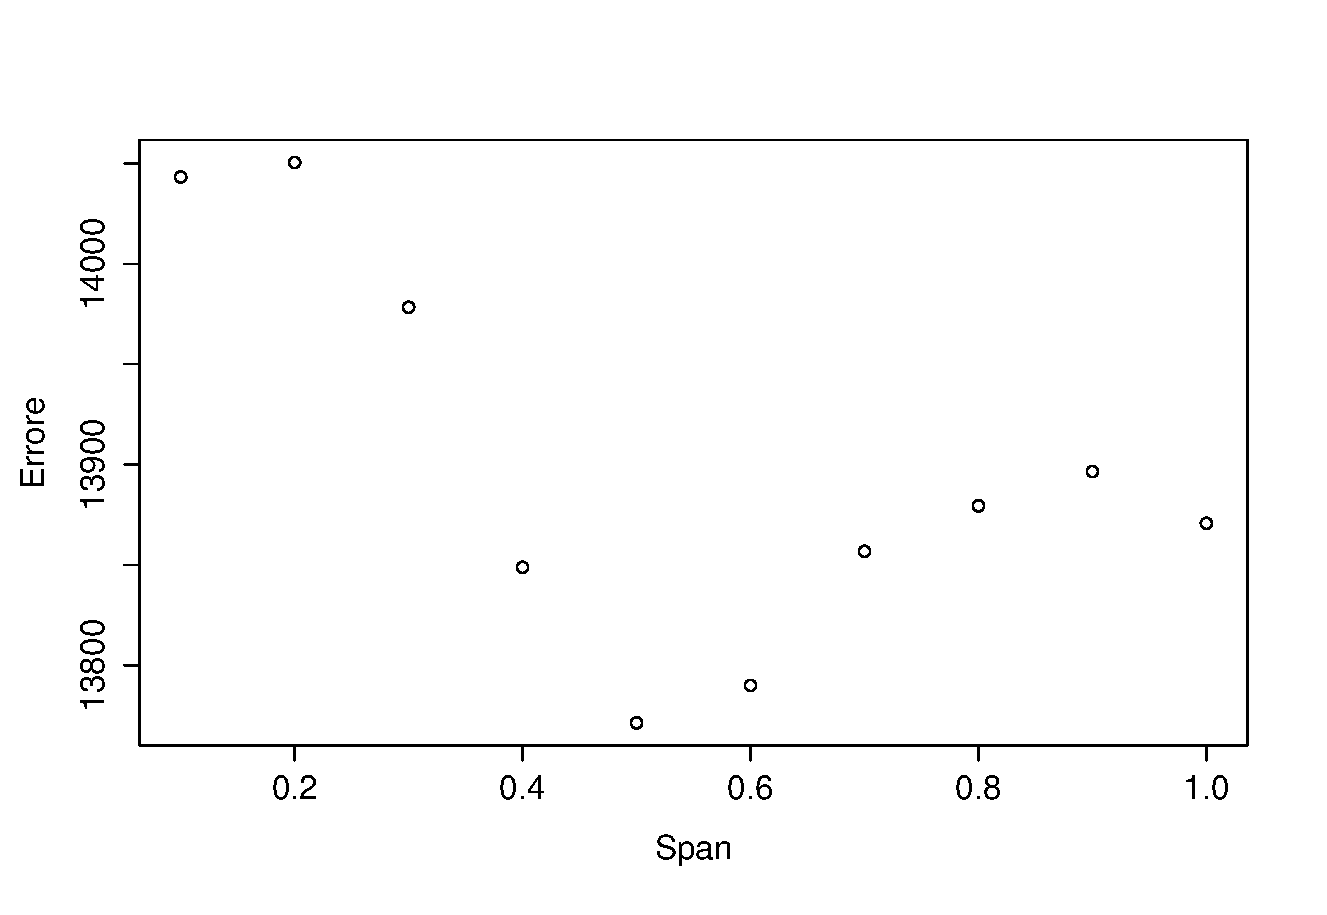
\includegraphics[width=.7\columnwidth]{images/non-linear/loess-error-span.eps}
  \caption{Curva dell'errore in funzione del parametro span}
  \label{fig:loess-optimal-span}
\end{figure}

\begin{figure}[H]
  \centering
  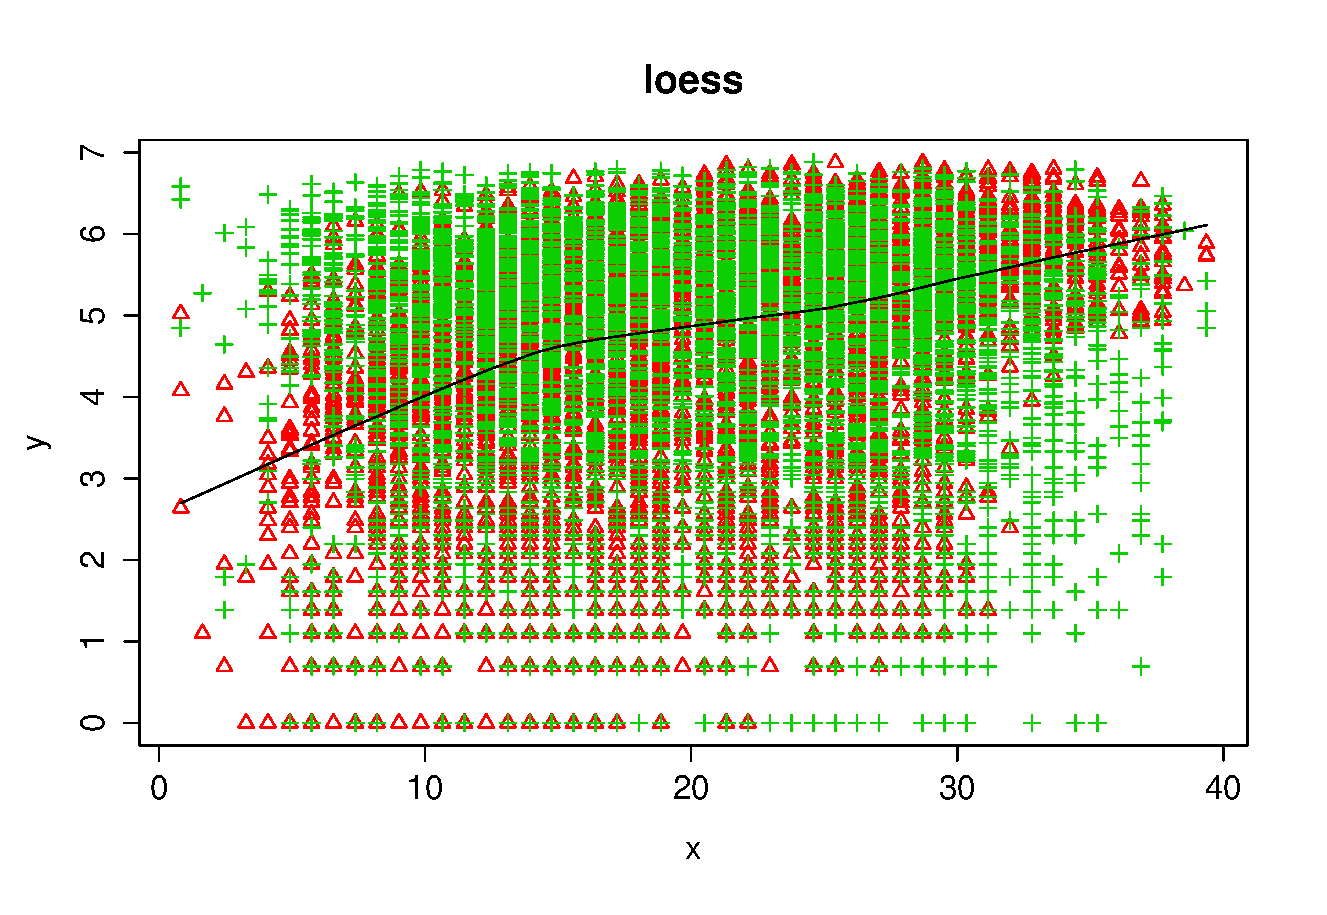
\includegraphics[width=.7\columnwidth]{images/non-linear/loess-draw.eps}
  \caption{Curva loess disegnata con il miglior span}
  \label{fig:loess-draw}
\end{figure}

\subsection{Spline di regressione}\label{doc:regression-splines}
Finora sono stati usati solamente modelli che, lineari o meno, erano costituiti
da una o più rette di regressione.

Con le spline si passa a curve che hanno tratti definiti da polinomi di grado
maggiore al primo: più precisamente, nel nostro caso verranno utilizzate
spline cubiche (con tratti definiti da polinomi di terzo grado).

Gli script che realizzano queste curve sono \texttt{regression-splines-temp.R}
(sez. \ref{sec:regression-splines-temp}) ed altri script non riportati perchè
sostanzialmente identici a questo.

Tali procedure utilizzano il comando \texttt{bs} di R, che genera spline con la
possibilità di impostare grado e numero di nodi.

\begin{figure}[H]
  \centering
  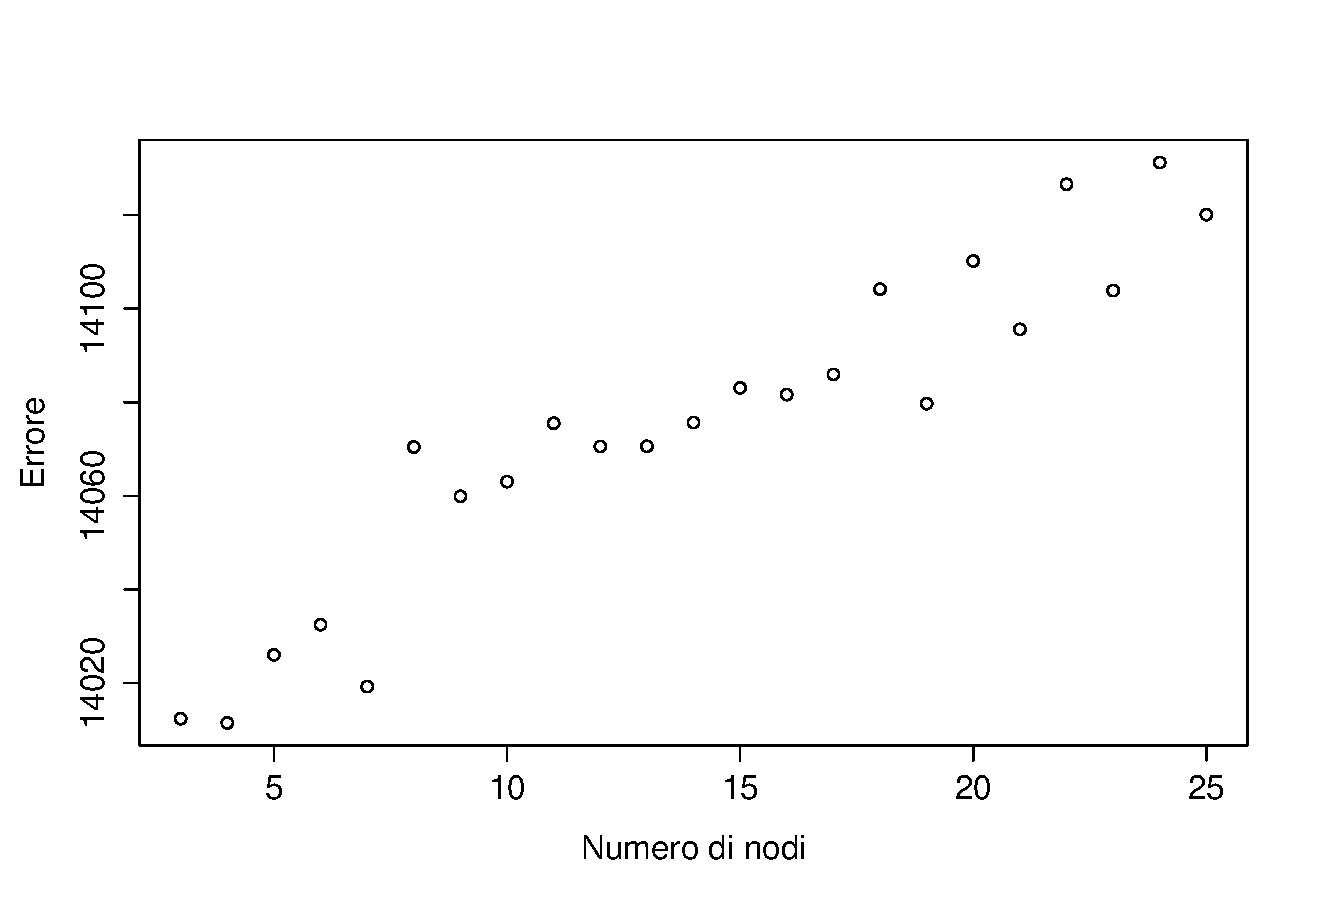
\includegraphics[width=.7\columnwidth]{images/non-linear/regression-splines-error-knots.eps}
  \caption{Curva dell'errore in funzione del numero di nodi}
  \label{fig:regression-optimal-knots}
\end{figure}

\begin{figure}[H]
  \centering
  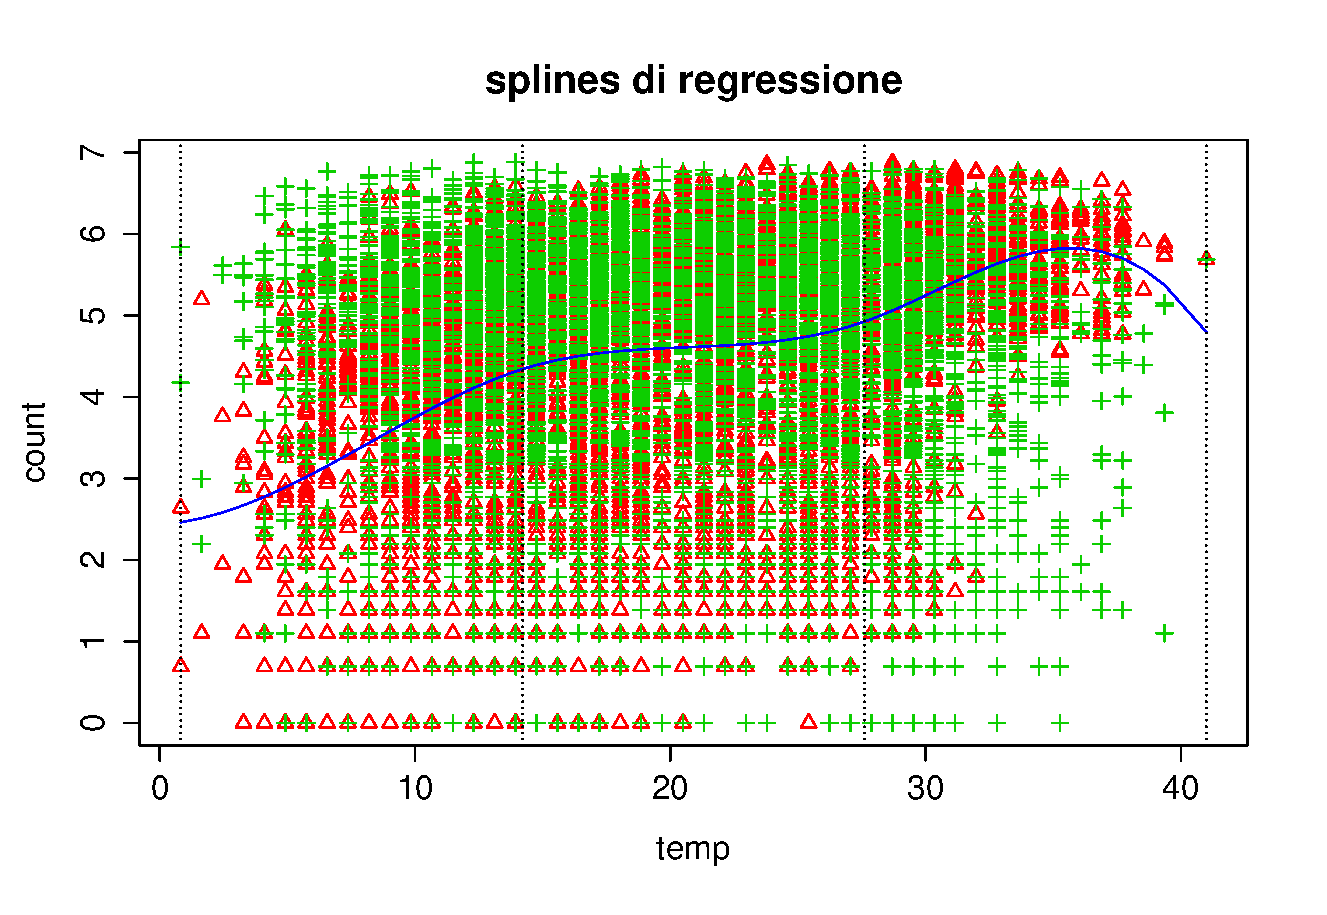
\includegraphics[width=.7\columnwidth]{images/non-linear/regression-draw.eps}
  \caption{Spline di regressione disegnata con il miglior numero di nodi}
  \label{fig:regression-draw}
\end{figure}
 % 0%

\appendix
\section{Script}\label{sec:script}

\subsection{populate.R}\label{sec:script-populate}
\begin{verbatim}
# Read tables
test = read.csv(file="data/test.csv")
train = read.csv(file="data/train.csv")

# DATETIME # Consider only hour
test$datetime = as.POSIXct(test$datetime)
test$datetime = strptime(test$datetime, "%Y-%m-%d %H:%M:%S")
test$datetime <- as.numeric(format(test$datetime, "%H"))
train$datetime = as.POSIXct(train$datetime)
train$datetime = strptime(train$datetime, "%Y-%m-%d %H:%M:%S")
train$datetime <- as.numeric(format(train$datetime, "%H"))

# HOURS # Treat hour of day as a qualitative covariate
test$datetime = factor(test$datetime)
train$datetime = factor(train$datetime)

# SEASONS # Treat as qualitative covariate
# summer
train$season.summer = rep(0,length(train$season))
train$season.summer[train$season == 2] = 1
test$season.summer = rep(0,length(test$season))
test$season.summer[test$season == 2] = 1
# fall
train$season.fall = rep(0,length(train$season))
train$season.fall[train$season == 3] = 1
test$season.fall = rep(0,length(test$season))
test$season.fall[test$season == 3] = 1
# bring all to 0 except spring
test$season[test$season == 2] = 0
test$season[test$season == 3] = 0
test$season[test$season == 4] = 0
train$season[train$season == 2] = 0
train$season[train$season == 3] = 0
train$season[train$season == 4] = 0

# COSTANTS # Some constants
columns = colnames(test)
MAX_P_DEGREE = 30
F1 = as.formula(paste("log(train$count)~",paste(names(train[-c(10:12)]), collapse="+")))

# LIFT-ROC # Import lift-roc script
source("scripts/lift-roc1.R")

\end{verbatim}

\subsection{linearModel.R}\label{sec:script-linear-model}

\begin{verbatim}
if(!is.factor(train$datetime))
  train$datetime = factor(train$datetime)
r2 = rep(0,length(columns)); fstatistic = rep(0,length(columns))

for(i in 1:length(columns)) {
  print(columns[i])
  myCol = train[columns[i]]
  train.lm = lm(log(train$count)~., data = myCol)
  r2[i] = summary(train.lm)$r.squared
  fstatistic[i] = summary(train.lm)$fstatistic[1]
  print(paste(columns[i], "has R-squared:", r2[i], " and F-statistic: ", fstatistic[i]))
}

best = 1
for(i in 2:length(columns)) {
  if(fstatistic[i] > fstatistic[best])
    best = i
}

print(paste(columns[best], "has best F-statistic:", fstatistic[best]))
print(paste(columns[best], "will be used to calculate the linear model w/ 1 variable"))

train.lm = lm(log(train$count) ~ ., data = train[columns[best]])

already_present = c(columns[best])
source("scripts/linear_model_forward_steps.R")
print(already_present)

#clean
rm(i)
rm(best)
rm(r2)
rm(fstatistic)
rm(already_present)
rm(myCol)
\end{verbatim}

\subsection{linear\_model\_forward\_steps.R}
\label{sec:script-linear-model-fwd-steps}

\begin{verbatim}
best_aic = AIC(train.lm)
#already_present = c(already_present,42)

for(i in 1:length(columns)) {
  if(columns[i] %in% already_present)
    next
  myFrame = train[,c(already_present,columns[i])]
  train.lm2 = lm(log(train$count) ~ .,data = myFrame)
  
  aicCur = AIC(train.lm2)
  #myAnova = anova(train.lm,train.lm2)
  #print(columns[i])
  #str(myAnova$`Pr(>F)`)
  if(aicCur < best_aic) {
    best_aic = aicCur
    best = i
  }
}

if(best_aic < AIC(train.lm)) {
  already_present = c(already_present,columns[best])
  myFrame = train[,c(already_present)]
  train.lm = lm(log(train$count) ~ .,data = myFrame)
  print(paste(columns[best], "column has been added to our linear model"))
  source("scripts/linear_model_forward_steps.R")
}

#clean
if(exists("myFrame"))
  rm(myFrame)
if(exists("myAnova"))
  rm(myAnova)
if(exists("best_aic"))
  rm(best_aic)
if(exists("aicCur"))
  rm(aicCur)
\end{verbatim}

\subsection{KalmanFilter.R}\label{sec:script-kalman}
\begin{verbatim}
indexes = sample(1:NROW(train),length(train$count)-10)

Aprimo = train[indexes,columns]
y = log(train[indexes,"count"])
X = model.matrix(~., data=Aprimo)

V = diag(1,ncol(X),ncol(X))
beta = matrix( c( mean(y[1]), rep(0, ncol(X) - 1) ), ncol(X), 1 )

beta.storia = matrix(NA, nrow(X), ncol(X))
beta.storia[1,] = beta

for(i in 1 : NROW(X)) {
  H = 1 / (1 + t(X[i,]) %*% V %*% X[i,] )
  beta = beta + H[1] * (V %*% X[i,] %*% (y[i] - t(X[i,] %*% beta)) )
  V = V - H[1] * (V %*% X[i,] %*% t(X[i,]) %*% V )
  beta.storia[i,] = beta
}

beta = matrix(beta)
rownames(beta) = colnames(X)

X11()
par(mfrow = c(3,1))
plot(beta.storia[,1], type="l")
plot(beta.storia[,2], type="l")
plot(beta.storia[,3], type="l")

rm(Aprimo)
rm(H)
rm(V)
rm(X)
rm(i)
rm(y)
rm(indexes)
rm(beta.storia)
\end{verbatim}

\subsection{MySM\_temp.R}\label{sec:mySM-temp}
\begin{verbatim}
# LOCAL REGRESSION #
# Load 'sm' library
library(sm)

# Set 'temp' as covariate and 'count' as response
x = train$temp
y = log(train$count)

# Choose h interval
#interv = 10:100
#divisions= 10
#interv = 100:200
#divisions= 100
#interv = 1700:2000
#divisions= 1000
interv = 18500:19000
divisions= 10000

# Draw plot in which 'count' is function of 'temp'
plot(x,y,col=3,pch=3)

# Run several times local regression and store prediction errors
val = matrix(NA, length(interv),1)
for (i in interv) {
  inc = i / divisions
  sm1 = sm.regression(x,y,h=inc,add=TRUE,ngrid=120,col=2)
  val[i-min(interv)] = sum((y[1:120]-sm1$estimate)^2)
}

# Draw errors as a function of h values
plot((interv)/divisions,val)

# Find best h
val = val[1:(length(val)-1)]
i = which(val == min(val))
optimal_h = interv[i]/divisions

# Clean workspace (but keep best h)
rm(divisions)
rm(i)
rm(inc)
rm(interv)
rm(sm1)
rm(x)
rm(val)
rm(y)
\end{verbatim}

\subsection{drawOptimalSM\_temp.R}\label{sec:drawSM-temp}
\begin{verbatim}
# DRAW LOCAL REGRESSION #
# Set 'temp' as covariate and 'count' as response
x = train$temp
y = log(train$count)

# Draw local regression with optimal h
plot(x,y,col=3,pch=3)
sm1 = sm.regression(x,y,h=optimal_h,add=TRUE,ngrid=120,col=2)

# Clean workspace
rm(x)
rm(y)
\end{verbatim}

\subsection{loess\_temp.R}\label{sec:loess-temp}
\begin{verbatim}
# LOESS #
# Get indexes for training & test set
indexes = sample(1:length(train$count), size=length(train$count)/2)
indexes.v = sample(setdiff(1:length(train$count), indexes))
column = "temp"

# Get actual training & test set
x = train[column]
x.v = x[indexes.v,column]
x = x[indexes,column]
y = log(train$count)
y.v = y[indexes.v]
y = y[indexes]

# Find best span by X-validation
nummin = 1
num = 10
val = matrix(NA,num,2)
for(i in nummin:num) {
  k=i/10
  val[i,1] = k
  lo1 = loess(y~x,span=k)
  val[i,2] = sum((y.v-predict(lo1))^2)
}

# Show error as a function of span
plot(val[nummin:num,1],val[nummin:num,2],xlab="Span",ylab="Errore")
print(val[nummin:num,])
optimal_span = min(val[,2])
optimal_span = val[,1][val[,2] == optimal_span]
print(paste("Optimal span is",optimal_span))
cat("Premere <Enter>"); readline()

# Draw loess with best span
lo1 <- loess.smooth(x,y,span=optimal_span)
plot(x,y,pch=2,col=2,main="loess")
points(x,y.v,pch=3,col=3)
lines(lo1)

# Clean workspace
rm(i)
rm(indexes)
rm(indexes.v)
rm(h)
rm(lo1)
rm(num)
rm(nummin)
rm(val)
rm(x)
rm(x.v)
rm(y)
rm(y.v)
\end{verbatim}

\subsection{regression-splines-temp.R}\label{sec:regression-splines-temp}
\begin{verbatim}
# REGRESSION SPLINES #
# Load 'splines' library
library(splines)

# Get indexes for training & test set
indexes = sample(1:length(train$count), size=length(train$count)/2)
indexes.v = sample(setdiff(1:length(train$count), indexes))
str(indexes)
str(indexes.v)

# Get actual training & test set
x = train$temp
str(x)
x.v = x[indexes.v]
x = x[indexes]
y = log(train$count)
y.v = y[indexes.v]
y = y[indexes]

# Plot training (red) & test (green) set
plot(x,y,pch=2,col=2,main="splines di regressione")
points(x,y.v,pch=3,col=3)

# Draw regression spline of arbitrary length
xi = seq(min(x),max(x),length=13)
xx = sort(c(x,xi[2:(length(xi)-1)]))
m1 = lm(y~bs(x,knots=xi[2:(length(xi)-1)],degree=3))
fit1 = predict(m1,data.frame(x=xx))
lines(xx,fit1)
# Draw splines intervals
for(i in 1:length(xi)) {
  abline(v=xi[i], lty=3)
}

# Find best number of knots by X-validation
nummin = 3
num = 25
val = matrix(NA,num,2)
for (i in nummin:num){
  h = i
  val[i,1] = h
  xi= seq(min(x),max(x),length=i+2)
  xx = sort(c(x,xi[2:(length(xi)-1)]))
  m1 = lm(y~bs(x,knots=xi[2:(length(xi)-1)],degree=3))
  
  val[i,2] = sum((y.v-predict(m1))^2)
}

# Show error as a function of number of knots and find best #knots
plot(val[nummin:num,1], val[nummin:num,2],xlab="Numero di nodi",ylab="Errore")
print(val[nummin:num,])
val = na.omit(val)
bestVal = min(val[,2])
pos = val[,1][val[,2]==bestVal]
print(paste("Wow",bestVal,"in position",pos))
cat("Premere <Enter>"); readline()

# Draw spline with best number of knots
plot(x,y,pch=2,col=2,main="splines di regressione",xlab="temp",ylab="count")
points(x,y.v,pch=3,col=3)
xi<-seq(min(x),max(x),length=pos)
xx<-sort(c(x,xi[2:(length(xi)-1)]))
m1<-lm(y~bs(x,knots=xi[2:(length(xi)-1)],degree=3))
fit1<-predict(m1,data.frame(x=xx))
lines(xx,fit1,col=4)
# Draw splines intervals
for(i in 1:length(xi)) {
  abline(v=xi[i], lty=3)
}

# Clean workspace
rm(bestVal)
rm(fit1)
rm(h)
rm(i)
rm(indexes)
rm(indexes.v)
rm(m1)
rm(num)
rm(nummin)
rm(pos)
rm(val)
rm(x)
rm(x.v)
rm(xi)
rm(xx)
rm(y)
rm(y.v)
\end{verbatim}

\subsection{smoothing-splines-temp.R}\label{sec:smoothing-splines-temp}
\begin{verbatim}
# SMOOTHING SPLINES #
# Load 'sm' library
library(sm)

# Get indexes for training & test set
indexes = sample(1:length(train$count), size=length(train$count)/2)
indexes.v = sample(setdiff(1:length(train$count), indexes))
column = "temp"

# Get actual training & test set
if(column == "datetime")
  x = as.numeric(train[column])
x = train[column]
str(x)
x.v = x[indexes.v,column]
x = x[indexes,column]
y = log(train$count)
y.v = y[indexes.v]
y = y[indexes]

# Plot training (red) & test (green) set
plot(x,y,pch=2,col=2,main="Splines di lisciamento")
points(x,y.v,pch=3,col=3)

# Create a dataset in which means of response variable respective to
# covariates are stored
myFrame = data.frame(x,y)
levs = unique(x)
med = rep(0,length(levs))
i = 0
for(l in levs) {
  i = i + 1
  cnt = length(with(myFrame, y[x==l]))
  med[i] = sum(with(myFrame, y[x==l])) / cnt
}

# Save old x & y
x_old = x
y_old = y
x = levs;
y = med;

# Same thing for test set
myFrame = data.frame(x.v,y.v)
levs = unique(x.v)
med = rep(0,length(levs))
i = 0
for(l in levs) {
  i = i + 1
  cnt = length(with(myFrame, y.v[x.v==l]))
  med[i] = sum(with(myFrame, y.v[x.v==l])) / cnt
}

# Same as above
x.v = levs
y.v = med

# Draw a first spline, without specifying lambda
s1 <- smooth.spline(x,y)
lines(s1)
cat("premere <Enter>"); readline()

# Find best lambda by X-validation
nummin <- 1
num <- 100
val <- matrix(NA,num,2)
for (i in nummin:num){
  h=i/100
  val[i,1]<-h
  s1 <- smooth.spline(x,y,spar=h)
  val[i,2]<-sum((y.v-predict(s1)$y)^2)
}

# Plot error as a function of lambda and save best lambda
plot(val[nummin:num,1], val[nummin:num,2],xlab="Lambda",ylab="Errore")
val[nummin:num,]
val = na.omit(val)
bestVal = min(val[,2])
pos = val[,1][val[,2]==bestVal]
print(paste("Best:",bestVal,"in position",pos))
cat("premere <Enter>"); readline()

# Plot smoothing splines with best lambda
plot(x_old,y_old,pch=2,col=2,main="Splines di lisciamento",xlab=column,ylab="Bike sharing request")
points(x.v,y.v,pch=3,col=3)
s1 <- smooth.spline(x,y,spar=pos)
lines(s1)

# Clean workspace
rm(bestVal)
rm(cnt)
rm(h)
rm(i)
rm(indexes)
rm(indexes.v)
rm(l)
rm(levs)
rm(med)
rm(myFrame)
rm(num)
rm(nummin)
rm(pos)
rm(s1)
rm(val)
rm(x)
rm(x_old)
rm(x.v)
rm(y)
rm(y_old)
rm(y.v)
\end{verbatim}

\subsection{mars.R}\label{sec:mars-script}
\begin{verbatim}
# MARS #
# Load 'polspline' library
library(polspline)

# Get indexes for training & test set
indexes = sample(1:length(train$count), size=length(train$count)/2)
indexes.v = sample(setdiff(1:length(train$count), indexes))

# Get actual training & test set
x = train[columns]
y = train$count
x.v = x[indexes.v,]
x = x[indexes,]
y = log(train$count)
y.v = y[indexes.v]
y = y[indexes]

# Request MARS model
mars<-polymars(y,x)

# Predict response variable on test set and draw lift-roc plots
p6 = predict(mars,x.v)
a6<- lift.roc(p6, y.v, type="crude")

# Clean workspace
rm(a6)
rm(p6)
rm(indexes)
rm(indexes.v)
rm(x)
rm(x.v)
rm(y)
rm(y.v)
\end{verbatim}

\subsection{gam.R}\label{sec:gam-script}
\begin{verbatim}
# GAM #
# Load 'gam' library
library(gam)

# Get indexes for training & test set
indexes = sample(1:length(train$count), size=length(train$count)/2)
indexes.v = sample(setdiff(1:length(train$count), indexes))
Fgam = as.formula(paste("y~",paste(names(train[-c(10:12)]), collapse="+")))

# Get actual training & test set
x = train[columns]
x$datetime = as.numeric(x$datetime)
y = train$count
x.v = x[indexes.v,]
x = x[indexes,]
y = log(train$count)
y.v = y[indexes.v]
y = y[indexes]

# Request (and plot) GAM model
gam1 <-  gam(Fgam, family=gaussian, data=x)
summary(gam1)
plot(gam1, ask=T)

# Predict response variable on test set and draw lift-roc plots
p8 <- predict(gam1,newdata=x.v,type="response")
a8<- lift.roc(p8, y.v, type="crude")

# Clean workspace
rm(a8)
rm(Fgam)
rm(indexes)
rm(indexes.v)
rm(p8)
rm(x)
rm(x.v)
rm(y)
rm(y.v)
\end{verbatim}

\subsection{ppr.R}\label{sec:ppr-script}
\begin{verbatim}
# PROJECTION PURSUIT REGRESSION #
# Get indexes for training & test set
indexes = sample(1:length(train$count), size=length(train$count)/2)
indexes.v = sample(setdiff(1:length(train$count), indexes))

# Get actual training & test set
x = train[columns]
x$datetime = as.numeric(x$datetime)
y = train$count
x.v = x[indexes.v,]
x = x[indexes,]
y = log(train$count)
y.v = y[indexes.v]
y = y[indexes]

# Set upper bound for iterations on PPR
UB = 20
errors = rep(0,UB)

# Iterate by changing # of projections value
for(k in 1:UB) {
  ppr1 = ppr(y ~ ., data=x, nterms = k)
  mppr1 = pmax(predict(ppr1,newdata=x.v), .5)
  pPPR = predict(ppr1,newdata=x.v,type="response")
  errors[k] = sum((y.v-pPPR)^2)
  print(paste("Done PPR with k = ", k, "-- error: ", errors[k]))
}

# Find and plot best k value
bestK = which.min(errors)
print(paste("Index ", bestK, " has best error: ",errors[bestK]))
plot(1:UB, errors, xlab = "k", ylab="Errore")
cat("press <Enter>"); readline()

# Get best PPR
ppr1 = ppr(y ~ ., data=x, nterms = bestK)
pPPR = predict(ppr1,newdata=x.v,type="response")

# Plot lift-roc for best PPR
aPPR = lift.roc(pPPR, y.v, type="crude")

# Clean workspace
rm(aPPR)
rm(bestK)
rm(errors)
rm(indexes)
rm(indexes.v)
rm(k)
rm(mppr1)
rm(pPPR)
#rm(ppr1)
rm(UB)
rm(x)
rm(x.v)
rm(y)
rm(y.v)
\end{verbatim}

\subsection{neural-network.R}\label{sec:nnet-script}
\begin{verbatim}
# RETI NEURALI #
# Load 'nnet' library
library(nnet)

# Store formula that will be used to compute the neural network
Fnet = as.formula(paste("count~",paste(names(train[-c(10:12)]), collapse="+")))

# Get indexes for training & test set
indexes = sample(1:length(train$count), size=length(train$count)/2 + 1)
indexes.v = sample(setdiff(1:length(train$count), indexes))

# Get actual training & test set
x = train[c(columns,"count")]
x$datetime = as.numeric(x$datetime)
x.v = x[indexes.v,]
x = x[indexes,]

# Try to converge with 100 iterations and get predicted values
n1 = nnet(Fnet, data = x, decay = 0.0016, size = 5, maxit = 100)
pNN = predict(n1, newdata = x.v)

# Plot lift-roc for best PPR
lift.roc(pNN,x$count,type="crude")

# Clean workspace
rm(Fnet)
rm(indexes)
rm(indexes.v)
rm(x)
rm(x.v)
\end{verbatim}

\include{sections/images}

%----------------------------------------------------------------------------------------

\newpage % Start the article content on the second page, remove this if you have a longer abstract that goes onto the second page

\end{document}
